\documentclass{article}
\usepackage{pgfplots}
\usepgfplotslibrary{groupplots,dateplot}
\usetikzlibrary{patterns,shapes.arrows}
\pgfplotsset{compat=newest}
\usepackage{tikz}
\usetikzlibrary{shapes, arrows.meta, positioning}
\usepackage[utf8]{inputenc}
\usepackage{amsmath}
\usepgfplotslibrary{groupplots}
\usepgfplotslibrary{fillbetween}
\usetikzlibrary{arrows,decorations.pathmorphing,positioning,fit,trees,shapes,shadows,automata,calc}
\usetikzlibrary{patterns,arrows,arrows.meta,calc,shapes,shadows,decorations.pathmorphing,decorations.pathreplacing,automata,shapes.multipart,positioning,shapes.geometric,fit,circuits,trees,shapes.gates.logic.US,fit, matrix,arrows.meta, quotes}
\usetikzlibrary{backgrounds,scopes}

\begin{document}

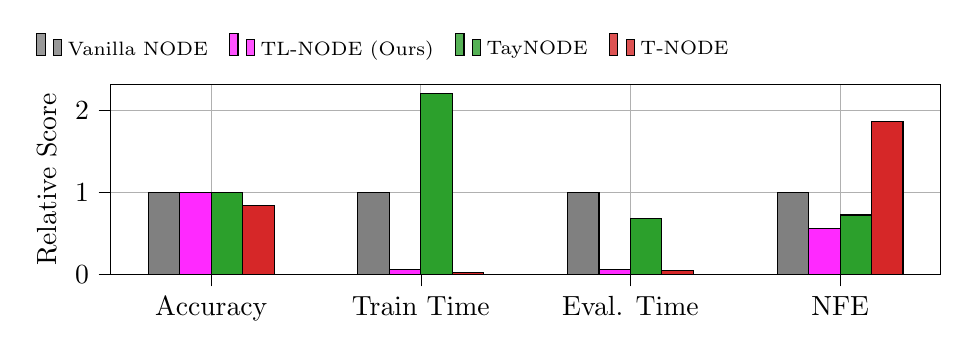
\begin{tikzpicture}

\definecolor{color0}{RGB}{128,128,128}
\definecolor{color1}{RGB}{255,41,255}
\definecolor{color2}{rgb}{0.172549019607843,0.627450980392157,0.172549019607843}
\definecolor{color3}{rgb}{0.83921568627451,0.152941176470588,0.156862745098039}

\begin{axis}[
height=4cm,
width=\columnwidth,
legend cell align={left},
legend columns = 4,
legend style={
    /tikz/every even column/.append style={column sep=0.2cm},
    font=\scriptsize,
  fill opacity=0.8,
  draw opacity=1,
  text opacity=1,
  at={(-0.1,1.3)},
  anchor=north west,
  draw=none,
},
tick align=outside,
tick pos=left,
x grid style={white!69.0196078431373!black},
xmajorgrids,
xmin=-0.255, xmax=3.705,
xtick style={color=black},
xtick={0.225,1.225,2.225,3.225},
xticklabels={Accuracy,Train Time,Eval. Time,NFE},
y grid style={white!69.0196078431373!black},
ylabel={Relative Score},
ymajorgrids,
ymin=0, ymax=2.321484375,
ytick style={color=black}
]

\draw[draw=black,fill=color0] (axis cs:-0.075,0) rectangle (axis cs:0.075,1);
\addlegendimage{ybar,ybar legend,draw=black,fill=color0}
\addlegendentry{Vanilla NODE}

\draw[draw=black,fill=color0] (axis cs:0.925,0) rectangle (axis cs:1.075,1);
\draw[draw=black,fill=color0] (axis cs:1.925,0) rectangle (axis cs:2.075,1);
\draw[draw=black,fill=color0] (axis cs:2.925,0) rectangle (axis cs:3.075,1);
\draw[draw=black,fill=color1] (axis cs:0.075,0) rectangle (axis cs:0.225,1.00367834883008);
\addlegendimage{ybar,ybar legend,draw=black,fill=color1}
\addlegendentry{TL-NODE (Ours)}

\draw[draw=black,fill=color1] (axis cs:1.075,0) rectangle (axis cs:1.225,0.068359375);
\draw[draw=black,fill=color1] (axis cs:2.075,0) rectangle (axis cs:2.225,0.0638036809815951);
\draw[draw=black,fill=color1] (axis cs:3.075,0) rectangle (axis cs:3.225,0.563636363636364);
\draw[draw=black,fill=color2] (axis cs:0.225,0) rectangle (axis cs:0.375,1.00153264534587);
\addlegendimage{ybar,ybar legend,draw=black,fill=color2}
\addlegendentry{TayNODE}

\draw[draw=black,fill=color2] (axis cs:1.225,0) rectangle (axis cs:1.375,2.2109375);
\draw[draw=black,fill=color2] (axis cs:2.225,0) rectangle (axis cs:2.375,0.687116564417178);
\draw[draw=black,fill=color2] (axis cs:3.225,0) rectangle (axis cs:3.375,0.727272727272727);
\draw[draw=black,fill=color3] (axis cs:0.375,0) rectangle (axis cs:0.525,0.841524471237356);
\addlegendimage{ybar,ybar legend,draw=black,fill=color3}
\addlegendentry{T-NODE}

\draw[draw=black,fill=color3] (axis cs:1.375,0) rectangle (axis cs:1.525,0.02625);
\draw[draw=black,fill=color3] (axis cs:2.375,0) rectangle (axis cs:2.525,0.0460736196319018);
\draw[draw=black,fill=color3] (axis cs:3.375,0) rectangle (axis cs:3.525,1.87);

\end{axis}

\end{tikzpicture}

\end{document}